\section{Efficiently updatable neural networks}

NNUE (\reflectbox{NNUE} Efficiently updatable neural network) is a neural network architecture that allows for very fast subsequent evaluations for minimal input changes. It was invented for Shogi by Yu Nasu in 2018 \cite{nnue:2018}, later adapted to Chess for use in Stockfish in 2019 and may be used in other board games as well. Most of the information described in this chapter can be found in the excellent Stockfish NNUE documentation \cite{nnue-pytorch}. \\

NNUE operates in the following priciples:

\begin{itemize}
    \item \textbf{Input sparsity}: The network should have a relatively low amount of non-zero inputs, determined by the chosen feature set. The presented feature sets have between 0.1\% and 2\% of non-zero inputs for a typical position. Having a low amount of non-zero inputs places a low upper bound on the time required to evaluate the network in its entirety, caused by some feature sets like \fs{HalfKP} when the king is moved.
    \item \textbf{Efficient updates}: From one evaluation to the next, the number of inputs changes should be minimal. This allows for the most expensive part of the network to be efficiently updated, instead of recomputed from scratch.
    \item \textbf{Simple architecture}: The network should be composed of a few and simple operators, that can be efficiently implemented with low-precision arithmetic in integer domain using CPU hardware. [no accelerators, aggresive quantization techniques]
\end{itemize}

[tradeoff between speed and accuracy]

\subsection{Architecture}


arquitectura half, dos capas
for this thesis...


\subsection{Efficient updates}


\begin{figure}[h]
\centering
\subfloat[\centering Linear layer]{{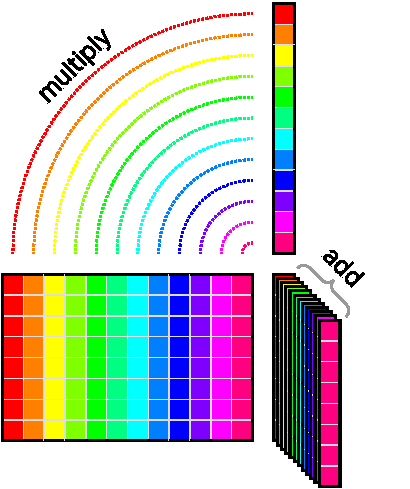
\includegraphics[width=5cm]{../assets/nnue/mv.pdf} }}%
\qquad
\subfloat[\centering Linear layer with sparse inputs]{{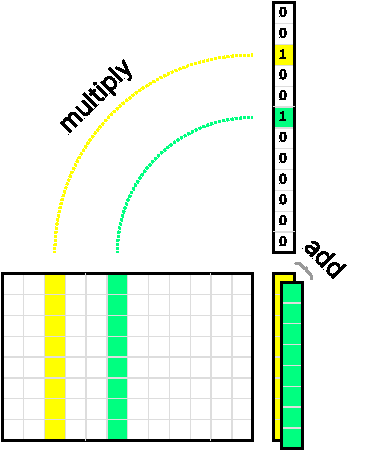
\includegraphics[width=5cm]{../assets/nnue/mvs.pdf} }}%
\caption{Linear layer operation comparison. Figures from \cite{nnue-pytorch}.}
\label{fig:linear_comparison}
\end{figure}


goes very well with incremental updates

pesada al principio y liviana al final, acumular filas de la primera capa en domove, undomove

\subsection{Stockfish quantization scheme}



\textbf{Rango de activación}: en el modelo original usamos ClippedReLU, asi que queremos que el rango vaya de 0..1 a 0..127.


Siendo $\bm{x}$, $\bm{w}$ y $\bm{b}$ los parámetros de una capa lineal sin cuantizar e $\bm{y}$ la salida de la misma, se tiene que:

\begin{equation}
\begin{aligned}
\bm{y} &= \bm{x} \bm{w} + \bm{b} \\
s_a s_w \bm{y} &= (s_a \bm{x}) (s_w \bm{w}) + s_a s_w \bm{b} \\
\end{aligned}
\end{equation}



\vspace{1cm}
$s_o ((s_a \bm{x}) (s_w \bm{w}) + s_a s_w \bm{b}) = s_a s_w s_o \bm{y}$



\subsection{Network sparsity}

o combinar con 3.2?
poner graficos con la sparsity de cada feature set, decir que es muy esparso todo y que se podría mejorar aún más
